\documentclass[a4paper,12pt]{article}
\usepackage[utf8]{inputenc}
\usepackage{amsmath}
\usepackage{amsfonts}
\usepackage{amssymb}
\usepackage{graphicx}
\numberwithin{equation}{section}
\renewcommand\thesubsection{\alph{subsection}}

%opening
\title{Quantum I HW5}
\author{Vince Baker}

\begin{document}

\maketitle

\section{Problem 1: Zeeman and Stark effects}
\subsection{}
The valence electron in a sodium atom will have nondegenerate N=3 states due to the screening effects of the lower-shell electrons.
With the 3P and 3D state energies lifted by 2 and 3 with respect to the 3S state, the $H_0$ matrix is: 
\begin{equation}
H_0=
\begin{bmatrix}
 0 & 0 & 0 & 0 & 0 & 0 & 0 & 0 & 0 \\
 0 & 2 & 0 & 0 & 0 & 0 & 0 & 0 & 0 \\
 0 & 0 & 2 & 0 & 0 & 0 & 0 & 0 & 0 \\
 0 & 0 & 0 & 2 & 0 & 0 & 0 & 0 & 0 \\
 0 & 0 & 0 & 0 & 3 & 0 & 0 & 0 & 0 \\
 0 & 0 & 0 & 0 & 0 & 3 & 0 & 0 & 0 \\
 0 & 0 & 0 & 0 & 0 & 0 & 3 & 0 & 0 \\
 0 & 0 & 0 & 0 & 0 & 0 & 0 & 3 & 0 \\
 0 & 0 & 0 & 0 & 0 & 0 & 0 & 0 & 3 \\
\end{bmatrix}
\end{equation}
\\
\subsection{}
With an external magnetic field applied along the z axis, the selection rules for $L_z$ are $m^{'}=m, \ell ^{'}=\ell $.
The $L_z$ matrix is :
\begin{equation}
L_z=
\begin{bmatrix}
 0 & 0 & 0 & 0 & 0 & 0 & 0 & 0 & 0 \\
 0 & 1 & 0 & 0 & 0 & 0 & 0 & 0 & 0 \\
 0 & 0 & 0 & 0 & 0 & 0 & 0 & 0 & 0 \\
 0 & 0 & 0 & -1 & 0 & 0 & 0 & 0 & 0 \\
 0 & 0 & 0 & 0 & 2 & 0 & 0 & 0 & 0 \\
 0 & 0 & 0 & 0 & 0 & 1 & 0 & 0 & 0 \\
 0 & 0 & 0 & 0 & 0 & 0 & 0 & 0 & 0 \\
 0 & 0 & 0 & 0 & 0 & 0 & 0 & -1 & 0 \\
 0 & 0 & 0 & 0 & 0 & 0 & 0 & 0 & -2 \\
\end{bmatrix}
\end{equation}
\\
\subsection{}
The matrix elements of $L_x$ can be calculated from the raising and lower operators $L^{\pm}$ by:
\begin{gather}
 L_+=L_x+iL_y\\
 L_-=L_x-iL_y\\
 L_x=\frac{1}{2}(L_++L_-)
\end{gather}

\begin{equation}
L_x=\frac{1}{2}
\begin{bmatrix}
 0 & 0 & 0 & 0 & 0 & 0 & 0 & 0 & 0 \\
 0 & 0 & \sqrt{2} & 0 & 0 & 0 & 0 & 0 & 0 \\
 0 & \sqrt{2} & 0 & \sqrt{2} & 0 & 0 & 0 & 0 & 0 \\
 0 & 0 & \sqrt{2} & 0 & 0 & 0 & 0 & 0 & 0 \\
 0 & 0 & 0 & 0 & 0 & \sqrt{4} & 0 & 0 & 0 \\
 0 & 0 & 0 & 0 & \sqrt{4} & 0 & \sqrt{6} & 0 & 0 \\
 0 & 0 & 0 & 0 & 0 & \sqrt{6} & 0 & \sqrt{6} & 0 \\
 0 & 0 & 0 & 0 & 0 & 0 & \sqrt{6} & 0 & \sqrt{4} \\
 0 & 0 & 0 & 0 & 0 & 0 & 0 & \sqrt{4} & 0 \\
\end{bmatrix}
\end{equation}
The energy spectrum of $L_z$ and $L_x$ are identical and are shown below:\\
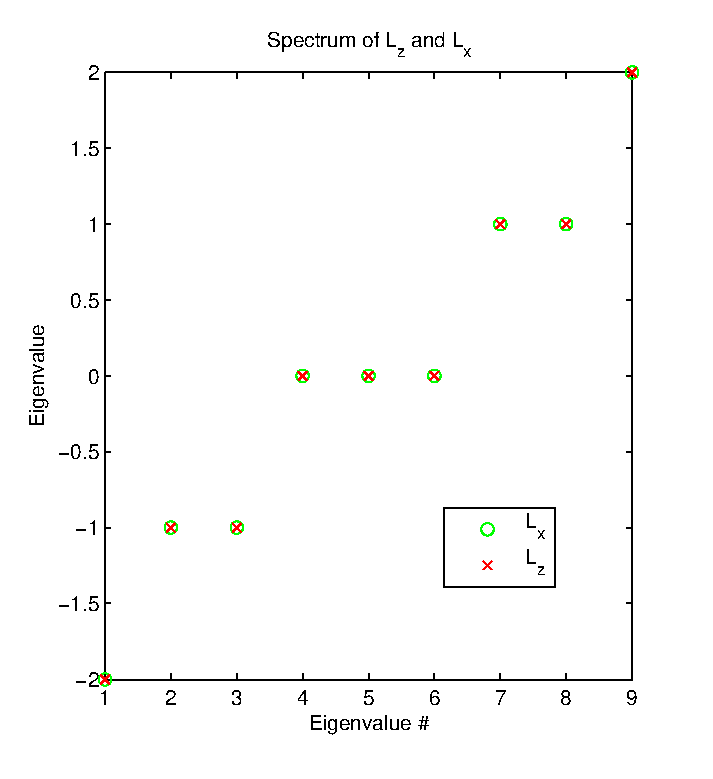
\includegraphics{Lx_Lz}
\\
\subsection{}
A uniform electric field is applied parallel to the z axis.
The Hamilton is:
\begin{equation}
-e|E|z=
\begin{bmatrix}
 0 & 0 & 1.633 & 0 & 0 & 0 & 0 & 0 & 0 \\
 0 & 0 & 0 & 0 & 0 & 1 & 0 & 0 & 0 \\
 1.633 & 0 & 0 & 0 & 0 & 0 & 1.1547 & 0 & 0 \\
 0 & 0 & 0 & 0 & 0 & 0 & 0 & 1 & 0 \\
 0 & 0 & 0 & 0 & 0 & 0 & 0 & 0 & 0 \\
 0 & 1 & 0 & 0 & 0 & 0 & 0 & 0 & 0 \\
 0 & 0 & 1.1547 & 0 & 0 & 0 & 0 & 0 & 0 \\
 0 & 0 & 0 & 1 & 0 & 0 & 0 & 0 & 0 \\
 0 & 0 & 0 & 0 & 0 & 0 & 0 & 0 & 0 \\
\end{bmatrix}
\end{equation}

\subsection{}
The energy spectrum of the sodium atom in electric and magnetic fields as a function of magnetic field angle $\theta$ is shown below:\\
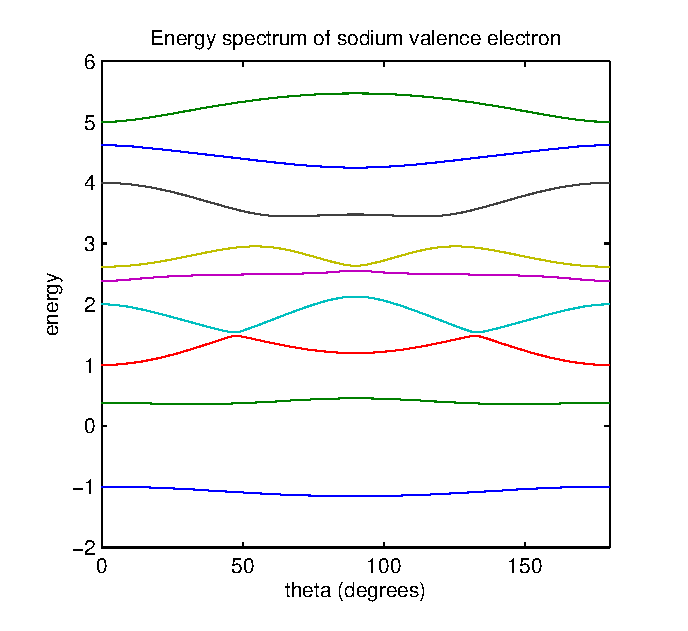
\includegraphics{Na_spectrum}
\\
\end{document}
